% to include:
% - pscore estimated is slightly less good for bias, much better for variance
% - extrapolation graph
% - edit dan's section
% - include para at top of variance section with ways of looking at
%   this, including anticipatory responce to A&I
\documentclass[11pt,titlepage]{article}
%\usepackage[notref]{showkeys}
\usepackage[reqno]{amsmath}
\usepackage{natbib}
\usepackage{amssymb}
\usepackage{epsfig}
\usepackage{comment}
\usepackage{url}
\usepackage[all]{xy}        
\usepackage{dcolumn}
\newcolumntype{.}{D{.}{.}{-1}}
\newcolumntype{d}[1]{D{.}{.}{#1}}
\usepackage{threeparttable,booktabs}
%\usepackage{times}
\usepackage{vmargin}
\setpapersize{USletter}
\topmargin=0in

% Shortcuts
\renewcommand{\P}{\text{P}}
\newcommand{\MC}{\multicolumn}
\usepackage{calc}
\newcounter{hours}\newcounter{minutes}
\newcommand{\printtime}{%
  \setcounter{hours}{\time/60}%
  \setcounter{minutes}{\time-\value{hours}*60}%
  \thehours :\theminutes}
%
\title{Matching as Nonparametric Preprocessing\\
  for Improving Parametric Causal Inference\thanks{Our thanks to Dan
    Carpenter and Jeff Koch for data; Olivia Lau for many helpful
    comments; and the National Institutes of Aging (P01 AG17625-01)
    and the National Science Foundation (SES-0318275, IIS-9874747) for
    research support.  Software to implement the methods in this paper
    is available from \texttt{http://GKing.Harvard.Edu/matchit}.}}

\author{Daniel E. Ho,\thanks{J.D.\ candidate, Yale Law School, Ph.D.\
    candidate, Department of Government, Harvard
    University. (Center for Basic Research in the Social Sciences, 34
    Kirkland, Cambridge MA 02138, USA;
    \texttt{http://www.people.fas.harvard.edu/\~\,deho},
    \texttt{Deho@Fas.Harvard.Edu}).}
%\and %
Kosuke Imai,\thanks{Assistant Professor, Department of Politics, Princeton
    University (Corwin Hall 041, Department of Politics, Princeton
    University, Princeton NJ 08544, USA;
    \texttt{http://www.princeton.edu/\~\,kimai},
    \texttt{KImai@Princeton.Edu}).}
%\and %
Gary King,\thanks{David Florence Professor of Government, Harvard
  University (Center for Basic Research in the Social Sciences, 34
  Kirkland Street, Harvard University, Cambridge MA 02138;
  \texttt{http://GKing.Harvard.Edu}, \texttt{King@Harvard.Edu}, (617)
  495-2027).}
%\and %
Elizabeth A. Stuart\thanks{Ph.D.\ Candidate, Department of Statistics,
  Harvard University. (Science Center 702, One Oxford Street,
  Cambridge, MA 02138, USA;
  \texttt{http://www.people.fas.harvard.edu/\~\,estuart},
  \texttt{Stuart@Stat.Harvard.Edu}).}}

\date{\today\ (\printtime)} 
\begin{document}\maketitle

\begin{abstract}
  The fast growing statistical literatures on matching methods in
  several disciplines offer the promise of causal inference without
  resort to the difficult-to-justify functional form assumptions
  inherent in commonly used parametric methods.  However, these
  literatures also suffer from many diverse and conflicting approaches
  to estimation, uncertainty, theoretical analysis, and practical
  advice.  In this paper, we propose a unified perspective on matching
  as a method of nonparametric preprocessing for improving parametric
  methods.  This approach makes it possible for researchers to
  preprocess their data (such as with the easy-to-use matching
  software we offer with this paper) and then to apply whatever
  familiar statistical techniques they would have used anyway.  Under
  our approach, instead of using matching to replace existing methods,
  we use it to make existing methods work better, such as by giving
  more accurate and considerably less model-dependent causal
  inferences.
\end{abstract}
%\baselineskip=1.57\baselineskip

\section{Introduction}

A new statistics literature has emerged in recent years, building on
advances in nonparametric, non-model-based inference, and focused
around diverse generalizations of different types of matching
estimators for causal inference.  The promise of this work is
considerable, as it promises more reliable and valid causal inferences
than is typical with the standard parametric regressions social
scientists usually run (regression, logit, etc.).  The new methods
make it possible to reduce or eliminate the functional form and other
assumptions of parametric models and to verify empirically rather than
assume critical modeling assumptions.

The statistical literature on matching has grown quite sophisticated
but, from the point of view of the practical researcher, it looks like
a cacophony of related but conflicting techniques, practices,
conventions, and rules of thumb.  Valid methods of computing standard
errors and confidence intervals are even more complicated, often not
used, and sometimes not available.  Many theoretical results do not
apply to real applications unless unknown theoretical quantities or
specifications are somehow divined, and so coherent guidelines for
practice are conflicting, absent, or based on clinical experience
rather than scientific proof.  Although matching now comprises a
substantial fraction of the empirical work in some disciplines, such
as epidemiology and medicine, the diversity of the substantive
applications, and the difficulties of the conflicting methodological
languages used to describe the same underlying concepts, has limited
the spread of these powerful techniques to much of the social
sciences.

In this paper, we attempt to unify this diverse literature so applied
researchers can make productive use of these new methods.  Our simple
unifying idea is to use these new nonparametric techniques not as
substitutes for our present parametric regression analyses, but
instead to use them to make our familiar parametric techniques work
better.  Under our inferential framework, analysts merely add a simple
preprocessing step to their data analysis procedures and then use
whatever models they were previously accustomed to using to analyze
the preprocessed data rather than the raw data.  All of the intuition,
diagnostics, and knowledge about our parametric procedures can then be
used as before.

Preprocessing data with matching in the way we propose improves
parametric analyses by making them considerably less dependent on
assumptions about functional forms and distributions.  Our
preprocessing approach has obvious advantages in terms of exposition,
pedagogy, and ease-of-use, since what we have already learned is not
discarded, but it also turns out to help bring some order and cohesion
to the conflicting methodological literature and to suggest some
relatively straightforward advice for empirical researchers seeking to
make causal inferences.  For example, when thought of in the way we
propose, the approach suggests a simple, standardized, and valid
approach to computing standard errors and confidence intervals for any
of the new techniques.  Our approach has also made it possible for us
to write easy-to-use software that implements all the ideas we discuss
in this paper; it is free and available at
http://gking.harvard.edu/matchit.

Our approach is similar in spirit to \citet{AbaImb04,RubTho00}, who
recommend (specific forms of) parametric adjustment following
matching, as well as \citet{HecIchTod98} who develop forms of matching
that are combined with semi-parametric (kernel weighting) analyses.
Applied researchers have intuitively chosen similar approaches, such as in
\citet{Rosenbaum86, GlaLevMye03}.  
It is also similar in spirit to methods in other areas that preprocess
data so that subsequent analyses can be improved without modififying
existing techniques, such as multiple imputation
\citep{Rubin87,KinHonJos01} and outlier and feature detection
\citep[][Ch.8]{Bishop95}.  

\section{Definition of Causal Effects}

The notation and ideas in this section parallel that in
\citet[][Section 3.1.1]{KinKeoVer94}, but key aspects of it originate
with many others, especially \citet{Rubin74} and \citet{Holland86}.
The most important idea in this literature is that a causal effect is
a theoretical quantity, defined independently of any empirical method
that might be used to estimate it from real data.  To explicate these
ideas, we use the running example from \citet[][Section
3.1.1]{KinKeoVer94}, where the goal is to estimate the electoral
advantage of incumbency for Democrats in the U.S.\ House of
Representatives.  That is, we only study Democratic incumbents and
define the treatment as when the Democratic Party nominates one of
these incumbents willing to run for a new term and the control as when
the Party nominates someone else to run in an open seat.

The unit of analysis in our example is therefore the congressional
district, which we label with the index $i$ ($i=1,\dots,n$).  In most
of the methodological literature on causal inference, researchers
simplify the exposition by considering only a single dichotomous
causal (or ``treatment'') variable.  We do the same and label it
$t_i$, which takes a value of 1 if unit $i$ receives the treatment and
0 if $i$ is untreated (the ``control condition'').  In our running
example, the treatment is whether the incumbent is given the party's
nomination in district $i$.  Projects with more complicated causal
variables can dichotomize (perhaps in several alternative ways) or use
more complicated methods \citep{ImaDyk03}.  Those with more than one
causal variable of interest can follow all the advice herein for one
variable at a time.

The observed outcome (or ``dependent'') variable is $y_i$, which in
our case is the Democratic proportion of the two-party vote in
congressional district $i$.  Finally, prior to the treatment decision,
each district $i$ has a variety of characteristics, some of which we
measure and collect in a vector denoted $X_i$.  (Whether preprocessing
or not, variables that are at least in part consequences of the
treatment variable should never be controlled for when estimating a
causal effect.)

To clarify our inferential goals, we begin by defining the ``realized
causal effect,'' which is the simplest definition available.  To
provide further familiarity with this concept, we briefly show the
close connections between this definition and the goals of the
substantively unrelated but mathematically closely related missing
data and ecological inference literatures.  We then generalize the
definition to include features of random causal effects that are
useful for our use of nonparametric methods of preprocessing for
parametric models.  Finally, we give specific causal estimates of
interest at the population level.

\paragraph{Realized Causal Effects}
Because of pretreatment differences among the districts (both
measured, $X_i$, and unmeasured), the causal effect may differ across
the districts.  As such, the definition of the causal effect exists at
the district level, but the definition does not otherwise require
reference to the pretreatment variables.

A causal effect is a function of \emph{potential outcomes}: let
$y_i(t_i=1)\equiv y_i(1)$ be the vote we would observe in district $i$
in say the 2008 election if in fact the Democratic incumbent receives
his or her party's nomination (i.e., $t_i=1$) and $y_i(t_i=0)\equiv
y_i(0)$ the vote the party would receive if the Democratic Party
nominates a nonincumbent ($t_i=0$).  The use of parentheses in this
notation denotes that the outcome is potential, and so not necessarily
observed, and that it depends on the value of the variable in
parentheses.  A key point is that the values of these potential
outcomes remain the same regardless of whether the treatment is in
fact applied in district $i$ or not.  However, since the Democratic
Party either will nominate ($t_i=1$) or will not nominate ($t_i=0$) an
incumbent to run in district $i$, we will observe either $y_{i}(1)$ or
$y_{i}(0)$ but not both.\footnote{We assume throughout that every unit
  within each treatment group receives the same treatment.  This
  assumption would be violated in our running example if the
  nomination the Democratic party gives to the incumbent in some
  districts means something different from that in other districts.
  We also assume that the treatment in one unit has no effect on the
  potential outcomes in any unit other than its own.  Together these
  two assumptions are sometimes known under the awkward name of the
  ``stable unit treatment value assumption'' or SUTVA
  \citep{Rubin74}.}

The difference between the two potential outcomes defines the simplest
realized (or in-sample) definition of a causal effect:
\begin{equation}
  \label{rce}
  \text{(Realized causal effect for unit $i$)} = y_i(1) - y_i(0).
\end{equation}
The fact that one of these potential outcomes is always a
counterfactual --- and thus is never known for certain no matter how
perfect the research design, experimental control, or number of
observations collected --- expresses what is known as the
``fundamental problem of causal inference'' \citep{Holland86}.

\paragraph{Connections to Missing Data and Ecological Inference}
Although causal inference is the ultimate goal of most research
programs in the social sciences, the inherent difficulty of this goal
is not always fully appreciated.  To clarify this issue, and to
further clarify the definition of causal effects, we now show how
causal inference is an extreme special case of two areas of statistics
that are widely, but incorrectly, perceived to be more difficult.

If district $i$ receives the treatment, we observe $y_i=y_i(1)$ but
not $y_i(0)$ and otherwise we observe $y_i=y_i(0)$ but not $y_i(1)$.
In this framework, causal inference can be thought of as a severe
missing data problem, where each unit has two relevant dependent
variables, $y_i(0)$ and $y_i(1)$, but one of which, $t_iy_i(0) +
(1-t_i)y_i(1)$, is always missing.  Moreover, since $y_i(0)$ and
$y_i(1)$ are never observed for the same units, we cannot use a known
relationship between the two to extrapolate to units where only one is
observed.  Making causal inferences is thus equivalent to imputing
missing data, using whatever external information is available.  As we
show below, this connection will prove useful in making the bridge
that connects nonparametric matching to parametric models.

Causal inference can also be thought of as an especially severe form
of ecological inference.  In ecological inference, we observe for each
observation the proportions representing the two marginals of a
$2\times 2$ contingency table (such as the proportion of people voting
and the proportion of people who are black) and the goal is to
estimate the unknown cell proportions (the proportion of blacks who
vote and the proportion of whites who vote).  We make the bridge by
referring to the known ($y_i$ and $t_i$) and potentially unknown
($y_i(0)$ and $y_i(1)$) quantities in both problems in the same
notation and pay attention to the order in which the information is
generated: In both problems, we imagine that $y_i(0)$ and $y_i(1)$
exist in nature before our research begins.  Then $t_i$ (the treatment
in causal inference or the row marginal in ecological inference) is
applied or otherwise becomes known.  Finally, we can calculate the
observed outcome $y_i$ deterministically via this simple accounting
identity:
\begin{equation}
  \label{id}
  y_i = t_iy_i(1) + (1-t_i)y_i(0).
\end{equation}
In ecological inference, by solving (\ref{id}) for one of the unknowns
as a linear function of the other and recognizing that proportions are
always constrained to the unit interval, we can put deterministic
bounds on both quantities of interest with certainty
\citep[][ch.5]{King97}.  In causal inference, we have the advantage of
always knowing one of the quantities exactly; however, because
(\ref{id}) cannot be solved for one of the unknowns (since it would
require dividing by $t_i$ or $1-t_i$, which includes zero) we have the
severe disadvantage of not knowing anything with certainty about the
other unknown.

Social scientists correctly think of missing data imputation and
ecological inference as difficult and hazardous areas of statistical
inference.  After all, both involve making inferences about patterns
in unobserved quantities by using patterns in observed data, with
nothing but optimistic assumptions guaranteeing that the former have
anything necessarily to do with the latter.  However, scholars should
be no less concerned when making causal inferences, as every causal
effect ever estimated involves essentially identical inferential
hazards.  If anything, the specific problems in making causal
inferences are even more difficult than most applications in these
other areas.  Moreover, whether using linear regressions, simple
descriptive differences in means, or complicated multiple equation
estimators, causal inference requires assumptions that are no easier
to justify than those in imputation or ecological inference.  In all
three areas the inferential target is not normally highly constrained
by the observed data and so substantive conclusions will usually
depend on unverifiable assumptions about the data generation process.
And so laying these assumptions bear as clearly as possible throughout
the process is essential.

\paragraph{Random Causal Effects} In order to make statistical
inferences, we imagine that the realized potential outcomes in
(\ref{rce}) are realizations of corresponding random variables (for
which we use the corresponding capital letters).  We do not require
that the data are sampled from some specific population, only that
there exists some data generation process that leads to the one
realization we see and could have led to some other realization.  This
logic then produces the random causal effect:
\begin{equation}
  \label{rance}
  \text{(Random Causal Effect for unit $i$)}  = Y_i(1) - Y_i(0),
\end{equation}
features of which we are interested in as alternative quantities of
interest.  For example, our second definition for the causal effect is
the mean causal effect, which is the average over repeated
hypothetical draws of the the random causal effect:
\begin{align}
  \label{meance}
  \text{(Mean Causal Effect for unit $i$)}
  &= E(\text{Random Causal Effect for unit $i$})\\
  &= E[Y_i(1) - Y_i(0)]\\ \notag &= \mu_i(1) - \mu_i(0),
\end{align}
where $E[Y_i(1)]\equiv\mu_i(1)$ and $E[Y_i(0)]\equiv\mu_i(0)$.

\paragraph{Average Quantities of Interest}
In most applications, we do not attempt to estimate the treatment
effect for each observation, and instead estimate the average over all
observations or some subset of observations.  This leads to two
choices for quantities of interest, for either realized and random
causal effects (we show them here for the latter).  First is the
population average treatment effect or ATE:
\begin{align}
  \label{pate}
  \text{ATE} = E[Y_i(1) - Y_i(0)] \\
  = \frac{1}{n}\sum_{i=1}^n[\mu_i(1) - \mu_i(0)],
\end{align}
which is the mean causal effect for unit $i$ averaged over all units
(so that the expected value operator in the first line averages over
the random potential outcomes for each unit as well as over units).

The alternative choice of a target quantity of interest is the average
treatment effect on the treated, or ATT:
\begin{align}
  \label{att}
  \text{ATT} = E[Y_i(1) - Y_i(0)|t=1] \\
  = \frac{1}{\sum t_i}\sum_{i:t_i=1}[\mu_i(1) - \mu_i(0)],
\end{align}
In our running example, this is the average causal effect in districts
in which the Democratic Party nominated the incumbent member of the
House.  From one perspective, we might want to know this treatment
effect on the treated (the ATT) since obviously this is the group of
districts where the treatment was applied.  In other words, the ATT is
the effect of the treatment actually applied.  Medical studies
typically use the ATT as the designated quantity of interest because
they often only care about the causal effect of drugs for patients
that receive or would receive the drugs.  For another example, in job
training programs, we are not normally interested in assinging
employed people to have this training.  In the social sciences, the
ATT is also a reasonable choice, but so is the average treatment
effect (the ATE).  In our running example, it is quite likely that if
an incumbent were nominated in districts in which he or she did not
actually receive the nomination that an incumbency advantage would
still exist, and whatever this effect is, it might be of substantive
interest.  In this paper, we usually focus on ATT as the quantity of
interest when it is conceptually or algebraically simpler, but we also
show how to compute the ATE.

\section{Data Collection Mechanisms}

We now describe the assumptions necessary for making causal inferences
in experimental and observational research.  Some version of these
assumptions, or some way to deal with the information in them, are
necessary no matter what statistical methods are used for estimation.
Any specific statistical method chosen will make additional
assumptions, but the ones discussed here affect essentially all
methods.

\subsection{Experimental}

Although true experiments are only very rarely conducted in political
science, they remain a useful ideal type for understanding other types
of research.  In addition, some of the assumptions necessary for valid
inference in experiments will be approximated by the preprocessing
procedures we suggest below.

Valid and relatively automatic causal inferences can be achieved via
classical randomized experiments (where by ``classical'' we refer to
the situation where randomness is complete and not merely applied
within categories of other variables).  Such experiments have three
critical features: (1) \emph{random selection} of units from a given
population to be observed, (2) \emph{random assignment} of values of
the treatment ($t_i$) to each observed unit, and (3) a \emph{large
  $n$}.

The first feature avoids selection bias by identifying a given
population and guaranteeing that the probability of selection from
this population is related to the dependent variable only by random
chance.  Combining this with the large $n$ from the third feature
guarantees that the chance that something will go wrong is vanishingly
small.

Random assignment in feature (2) guarantees the absence of omitted
variable bias even without any control variables included.  To see
this, recall that, under the usual econometric rules for omitted
variable bias, a variable $X_i$ must be controlled for if it is
causally prior to $t_i$, empirically related to $t_i$, and affects
$y_i$ conditional on $t_i$.  If, instead, one or more of the three
conditions do not hold, then $X_i$ may be omitted without any bias
resulting.  Random assignment guarantees that $t_i$ is unrelated to
\emph{any} $X_i$, whether measured or not, except by random chance.
Moreover, the large $n$ in condition (3) guarantees that this chance
is vanishingly small.

Experiments are a true ideal type, particularly in relation to most
social science research where almost all research fails to meet at
least one of the three features.  Even most social science lab
experiments have random assignment but no random selection and often a
small $n$.  Traditional survey research has what is intended to be
random selection (although with dramatically increasing nonresponse
rates and cell phone usage, this is a less plausible claim) and
certainly has a large $n$, but random assignment, except when the
treatment involves the wording of survey questions, is usually
impossible.

\subsection{Observational}

We define observational data colelction mechanisms as any process
generating data that does not meet all three of the features of a
classical randomized experiment.  Researchers trying to use the
experimental paradigm try to design research to meet all three
features discussed in the previous section.  Researchers analyzing
observational data are instead forced to make assumptions that, if
correct, help them avoid various threats to the validity of their
causal inferences.

In this paper, we shall assume data are selected in a manner that does
not generate selection bias.  Observations need not be selected at
random, as in an experiment, but the probability of selection must not
be correlated with the dependent variable $y$, after taking into
account the treatment $t$ and pre-treatment covariates, $X$.  Whether
this assumption is satisified by carefully considering and controlling
for the sample selection process or by changing the quantity of
interest to be that reflected by the sample, avoiding selection bias
is not a trivial matter, and it is the subject of a great deal of
concern and study in a large variety of methodological and substantive
literatures.  We mention it here to emphasize that all the well-known
concerns about selecting on the dependent variable should remain a
concern to researchers even when adopting our approach of
preprocessing data via nonparametric matching procedures.

We also assume that a researcher analyzing observational data has
sufficient information in their measured pre-treatment control
variables $X$ so that it is possible via \emph{some} method to make
valid causal inferences.  This is known in some fields as the absence
of omitted variable bias, so that $X_i$ must include all variables
that are causally prior to $t_i$, associated with $t_i$, and affect
$y_i$ conditional on $t_i$.  In other fields, this same condition is
known as ignorability, which means that $t_i$ and the potential
outcomes are independent after conditioning on $X_i$, and so we can
literally ignore all unobserved variables.  Ignorability is a strong
condition, but it is one about which social scientists are deeply
knowledgeable and which is the central methodological concern of many
substantive scholarly articles.  We emphasize this assumption to make
clear that our procedures contain no magic: They are unable to control
for variables that are not measured.

Assuming ignorability and the absence of selection bias still leaves
many assumptions to be made when choosing a specific statistical
inference method.  Results from these methods can still be biased,
unbiased, efficient, inefficient, and almost anything else, depending
on the analyst's choices.  We now focus on this point in the context
of commonly used parametric methods.

\section{Parametric Analysis Methods}

Researchers in the situation of knowing the parametric model that
generated their data, up to but not including some unknown parameters,
should specific and directly estimate this parametric model.
Preprocessing with matching procedures is suboptimal in this
situation.  Of course, few researchers with real observational data
sets in the social sciences have this kind of knowledge and as a
result some choices need to be made among the range of possible
parametric models.

We thus begin by specifying a single but general parametric model that
characterizes the range of models that researchers might choose from.
Indeed, the special cases of this model include almost all parametric
models that have been used in the social sciences.  First define the
stochastic component as $Y_i \sim p(\mu_i,\theta)$, for a specified
probability density $p(\cdot)$, mean $\mu_i$, and vector of ancillary
parameters $\theta$.  Then denote the systematic component as
$E(Y_i|t_i,X_i)\equiv\mu_i=g(\alpha + t_i\beta + X_i\gamma)$, for some
specified functional form $g(\cdot)$ and with intercept $\alpha$ and
coefficients $\beta$ and $\gamma$.  The ancillary parameters may also
be specified to vary over observations as a function of $X_i$ or other
covariates.  This framework includes all ``generalized linear models''
as well as many others.  For example, if $p(\cdot)$ is normal and
$g(c)=c$, we have linear regression; if $p(\cdot)$ is Bernoulli and
$g(c)=1/(1+e^{-c})$, the model reduces to a logistic regression.

We define the ATT in (\ref{att}) under this model by plugging in the
definitions of the potential outcomes from the systematic component,
with $t_i$ taking on values 1 and 0 respectively:
\begin{align}
  \label{matt}
  E(Y_i(1)|t_i=1,X) &\equiv \mu_i(1) = g(\alpha + \beta + X_i\gamma)\notag \\
  E(Y_i(0)|t_i=0,X) &\equiv \mu_i(0) = g(\alpha + X_i\gamma)
\end{align}
We can produce estimates of these quantities by assuming independence
over observations, and forming a likelihood function
\begin{equation}
  \label{lik}
  L(\alpha,\beta,\gamma,\theta|y) = \prod_{i=1}^n 
  p\left(y_i \mid g(\alpha + t_i\beta + X_i\gamma), \theta\right)
\end{equation}
the maximum of which gives parameter estimates.

We now turn to the difficulties in making causal inferences from
experimental vs.\ observational data under this general model.

\subsection{Experimental Data}\label{s:paraexp}

In experimental data, classical random assignment guarantees that
$T_i$ and (any observed or unobserved) $X_i$ are independent.  Since
stochastic independence implies mean independence, we can drop $X$ and
write $E[Y_i(1)|t_i=1,X]=E[Y_i(1)|t_i=1]$ and
$E[Y_i(0)|t_i=1,X]=E[Y_i(0)|t_i=1]$.  As such, we can simplify
(\ref{matt}) as
\begin{align}
  \label{smatt}
  E[Y_i(1)|t_i=1] &\equiv \mu_i(1) = g(\alpha + \beta)\notag \\
  E[Y_i(0)|t_i=0] &\equiv \mu_i(0) = g(\alpha)
\end{align}
and so the average treatment effect on the treated from (\ref{att})
becomes simply
\begin{equation}
  \label{satt}
  \text{ATT} = g(\alpha+\beta) - g(\alpha),
\end{equation}
which most importantly no longer has a summation sign over $i$.

The systematic components in Equations \ref{smatt} are now scalar
constants for all $i$.  This is a key result, since it means that
changing the definition of the functional form $g(\cdot)$ now amounts
to nothing more than a simple reparameterization.  Fortunately,
maximum likelihood is invariant to reparameterization --- meaning, for
example, that the MLE of $\alpha$ is the same as the square root of
the MLE of $\alpha^2$ \citep[][p.75-6]{King89} --- which implies that
no matter how $g(\cdot)$ is defined we get the same estimate of the
expected potential outcomes.\footnote{To rule out degenerate cases
  such as $g(a)=8$, we require that the image of $g(\cdot)$ and the
  potential outcomes be the same.} Moreover, given any chosen
stochastic component, this result holds for virtually any parametric
model, including all the special cases of the general model given
above.

Since the specific maximum likelihood estimator of the population mean
for most common probability densities is merely the sample mean, the
analysis of classical randomized experiments often comes down to
taking the difference in the sample means of $y$ for the treatment and
control groups.  But even if one chooses to run a parametric model,
the absence of model dependence means that the choice for a functional
form will not matter: The results will be the same no matter what the
choice for $g(\cdot)$ is.

\subsection{Observational Data} \label{s:paraobs}

In experiments, then, random assignment breaks the link between $T$
and $X$ and, by so doing, eliminates the problem of model dependence.
When analyzing observational data with parametric methods we are not
so fortunate.  We cannot reduce Equations \ref{att} to Equations
\ref{matt} and so are left having to model the full functional
relationship that connects the mean as it varies as a function of $t$
and $X$ over observations.  Since $X$ is typically multidimensional,
this is a surprisingly difficult task.

To see this point, which is known as the curse of dimensionality,
suppose for simplicity that we have a dependent variable and one
ten-category explanatory variable, and our goal is use linear
regression technology to estimate the functional relationship without
functional form assumptions.  To do this, we would represent the ten
categories with ten parameters (a constant and nine dummy variables or
10 mean indicator variables).  In contrast, the usual approach to
estimation is to assume linearity.  This enables us to enter not 10
indicator variables, but rather only a constant term and one slope
coefficient.  How do we get from ten parameters to only two?  Pure
assumption.  If we have some sense that the relationship is indeed
linear or close to linear, this is a good use of external information
to reduce the number of parameters that must be estimated.  If not,
then we still have the best linear approximation to the conditional
expectation function, but the relationship we estimate can be far off.
If we are running this regression for the purpose of estimating a
causal effect, then the treatment variable is also in the regression,
and its coefficient can be biased to any degree if the functional
relationship with the control variables is misspecified.

This problem quickly becomes more serious as the number of explanatory
variables increase.  For example, estimation without functional form
assumptions with two ten-category explanatory variables would require
not 20 parameters but 100.  In this case, the usual approach would
include a constant term and two slope coefficients, reducing 100
parameters to three by pure assumption.  And with multiple explanatory
variables, claims about external knowledge constraining the functional
form much become dubious.  In this example, by what theory would we
know that 97 parameters, representing every form of nonlinearity and
interaction, should be set to exactly zero?  Including a linear
interaction would not help much since it would merely add one more
parameter to estimate, and so we would still need to make assumptions
about the remaining 96 parameters.

The problem escalates very fast as the number of explanatory variables
increase.  With $v$ 10-category variables, we need $10^v$ parameters
for estimation in a regression framework without functional form
assumptions.  So five explanatory variables leads to a regression
model with 100,000 parameters, and the usual approach works by
estimating only a constant term and five slope coefficients and
restricting by assumption the remaining 99,994 parameters.  Nine such
explanatory variables leaves us with a model with one \emph{billion}
parameters, to be approximated by only the ten that we would estimate
under the traditional approach.  Eighty ten-category explanatory
variables would require a regression model with more parameters than
current estimates of the number of elementary particles in the
universe.

Estimating rather than making assumptions about all these extra
parameters is obviously not possible under the standard regression
approach, since social data sets do not come with anywhere near enough
observations.  We cannot avoid the problem with nonlinear or
non-normal statistical models, since these pose the same curse of
dimensionality as linear regression.  The assumption of ignorability,
which enables us to make the positivist assumption that we have have
measured and observe all necessary variables, is insufficient.

Instead, we are led to the inescapable conclusion that, in parametric
causal inference of observational data, many assumptions about many
parameters are frequently necessary, and only rarely do we have
sufficient external information to make these assumptions based on
genuine knowledge.  The frequent unavoidable consequence is high
levels of model dependence, but no good reason to choose one set of
assumptions over another.

% graph on interpolation and extrapolation

Some researchers surely respond to this diversity of possible models
by inadvertently choosing specifications that support their favored
hypotheses.  Current best practice is to forthrightly portray at least
some aspects of specification uncertainty in published work by giving
results for multiple specifications and evaluating how model dependent
the substantive results are.  But researchers rarely portray the full
sensitivity of their causal inferences to model specification, and
attempts to do so in many situations lead to nihilistic
conclusions.\footnote{Two approaches to this problem include extreme
  bounds analysis \citep{Leamer78}, which is a somewhat standardized
  way to portray model dependence, and Bayesian model averaging
  \citep{HoeMadRaf99,ImaKin04}, which is intended to draw inferences
  by appropriately combining inferences from models with different
  specifications.}

\section{Nonparametric Preprocessing} \label{s:nonparpreproc}

The goal of matching in general and our specific nonparametric
preprocessing approach is to adjust the data prior to the parametric
analysis so that (1) the relationship between $t_i$ and $X_i$ is
eliminated or reduced and (2) no bias and little inefficiency is
induced.  If we are able to adjust the data so that $t_i$ and $X_i$
are completely unrelated, so that the control and treatment groups are
identical with respect to $X$, we will have moved a good deal of the
way from Section \ref{s:paraobs} to Section \ref{s:paraexp}.  An
assumption of ignorability will still be necessary, but we will no
longer need to model the full parametric relationship between the
dependent variable and the multidimensional $X_i$.  We will also have
eliminated an important source of model dependence in the resulting
parametric analysis stemming from the functional form specification
and the curse of dimensionality.  For data sets where preprocessing
reduces the extent of the relationship between $t_i$ and $X_i$, but is
unable to make them completely independent, model dependence is not
eliminated but will normally be greatly reduced.  Indeed, if
nonparametric preprocessing results in no reduction of model
dependence, then it is likely that the data have little information to
support causal inferences by any method, which of course would also be
useful information.

But how can we adjust the data without inducing bias in our causal
estimates?  The key to this problem is that the fundamental rule for
avoiding selection bias --- do not select on the dependent variable
--- does not prevent us from selecting observations on the explanatory
variables ($t_i$ or $X_i$).  Random or other physical assignments in
experiments by the investigator and stratified sampling in surveys are
examples of data collection mechanisms that select observations given
chosen values of the explanatory variables.  But we can also select,
duplicate, or selectively drop observations from an existing sample
without bias, as long as we do so using a rule that is a function only
of $t_i$ and $X_i$.  Our preprocessed dataset will therefore include a
selected subset of the observed sample for which $t_i$ and $X_i$ are
unrelated, or in other words for which this relationship holds:
\begin{equation}
  \label{balance}
  p(X|t=1) = p(X|t=0).
\end{equation}

The simplest way to satisfy (\ref{balance}) is to use \emph{one-to-one
  exact matching}.  The idea is to match each treated unit with one
control unit for which the values of $X_i$ are identical.  Our
preprocessed dataset thus is the same as the original dataset with any
unmatched units discarded, and $t_i$ and $X_i$ are now independent.
If enough matches are available, this procedure eliminates all
dependence on the functional form in the parametric analysis.  It is
also highly intuitive, since it directly parallels an experiment where
we find pairs of units that are identical in all observable ways and
assign one from each pair to be treated and the other to be a control.
Then no matter what effect $X_i$ has on $y$, we can ignore it entirely
since $X_i$ is literally held constant within each pair of units.

Although one-to-one exact matching can eliminate model dependence and
any bias from incorrect assumptions made during the parametric stage
of analysis, it has the disadvantage in many applications of not
generating many matches.  The problem is of course most severe if
$X_i$ is high dimensional (another effect of the curse of
dimensionality) or contains continuous variables.  The result may then
be a preprocessed data set with very few observations that results in
a parametric analysis with large standard errors.  In this situation,
we may have reduced model dependence and the potential for bias but
decreased efficiency and as a result increased mean square error.  If
this occurs in practice, those in the matching literature tend to
sacrifice some bias reduction for the increased efficiency that comes
from having more observations in the preprocessed dataset.  In our
approach, sacrificing bias reduction only affects the preprocessing
stage, and our second stage parametric analysis has a chance to
eliminate the remaining bias.  We therefore now turn to a menu of
matching procedures that enable researchers to satisfy (\ref{balance})
as closely as possible while still generating a preprocessed dataset
with enough observations.

\section{Choosing a Matching Procedure}

In this section, we offer a step by step guide to navigating the wide
variety of matching procedures proposed throughout the statistics,
economics, epidemiology, medical, and biostatistics literatures.
These are young and fast-growing areas, and so we try to distill the
current collective wisdom when one is available or, when not, suggest
an approach that is at least widely recognized as reasonable.  For
detailed reviews of the technical literatures, and other matching
procedures, see \citep{Imbens04,Rosenbaum02,Stuart04} and
the detailed user's guide to the software that accompanies this paper
(see Appendix \ref{s:matchit}).

The goal of matching is to improve \emph{balance}, the degree to which
the treatment and control $X$ distributions resemble each other, while
not losing too many observations in the process.  The main diagnostic
of success is also balance (as well as the number of observations
remaining).  We judge balance at first by taking the difference in the
treatment and control group means or full histograms for each variable
in $X$.  These can be supplemented by comparing the means of the
squares and cross-products of the variables and higher order moments
or with more dimensions.

In our quest for better balance, any number of matching procedures can
be tried, with the final preprocessed data set the one with the best
balance.  To ensure that selection during preprocessing is only on
$X$, so no bias is induced, the outcome variable $y$ should not be
examined during the preprocessing stage.  As long as $y$ is not
consulted, preprocessing cannot result in stacking the deck one way or
another.  This is similar to what is typically done in a randomized
experiment: Before collecting the outcome data, if an undesirable
randomization is obtained (e.g., all men in the treated group and all
women in the control group), the randomization is repeated at will
until a better one is obtained \citep[see][]{Rubin01}.

We recommend that preprocessing be composed of four key steps,
followed by standard parametric modeling of the preprocessed data set.
We describe this procedure for the ATT, and so the matching is
designed to choose control units that look most like the treated
units.  We generally think of choosing for each treated unit the
control unit that looks the most similar to it, but variations are
possible.

\paragraph{1. Select Covariates}  
Include all variables in $X$ that would have been included in your
parametric model without preprocessing.  By the usual rules of
avoiding omitted variable bias these should include all variables that
may affect the treatment assignment and the dependent variable.  More
with matching than in parametric techniques, including variables only
weakly related to treatment assignment will usually reduce bias more
than they will increase variance and so should normally be included
\citep{RubTho96, HecIchSmi98}.  To avoid post-treatment bias, be sure to
exclude variables affected by the treatment variable (\cite{FraRub02},
\cite{Greenland03}, \citet{KinZen04}).

If all the variables in $X_i$ are categorical, try exact matching in
Step 2.  Otherwise, try propensity score matching in Step 3.
  
\paragraph{2. Try Exact Matching}  
Match each treated unit to all control units with exactly the same
covariate values.  This procedure is thus more general than one-to-one
matching, since we use as many control units as are available for each
treated unit.

If a large number of units were matched, then we have have exact
balance little inefficiency: go to the parametric analysis.  If
insufficient matches could be found, either repeat the exact matching
with fewer covariates or switch to propensity score matching,
described in Step 3.  In the former, we balance the included variables
but do not balance at all on the rest, which might not be exactly
balanced in the final analysis.  In the latter, we approximately match
on all the covariates.

\paragraph{3. Use Propensity Score Matching}  
The first step in this procedure is to summarize all the variables in
$X$ with a single variable called the \emph{propensity score}
\cite{RosRub83}.  The propensity score is the true probability of
unit $i$ receiving treatment, given the covariates $X_i$, $e_i(X_i) =
P(t_i=1 | X_i)$.  It is usually estimated via a logistic regression of
$t_i$ on a constant term and $X_i$.  The propensity score is central
to modern matching methods, but the present state of statistical
theory means that its role as a theoretical idea differs markedly from
its role in practice.  Understanding this disconnect, an explanation
of which to our knowledge has not explicitly appeared before in the
literature, is fundamental to making good practical use of this
important concept.

From a theoretical perspective, the true propensity score is valuable
because it is a ``balancing score,'' meaning that if a group of units
have similar propensity score distributions, then the covariates will
be balanced in the treated and control groups on all variables in $X$.
In addition, if the treatment assignment is ignorable given the
covariates $X_i$, then it is also ignorable given only the propensity
score.  This means that matching can be done using just the
one-dimensional propensity score, instead of all of the covariates
$X$.  Using the true propensity score in this way thus would seem to
solve the curse of dimensionality for matching.

In practice, however, we do not know the true propensity score (except
perhaps in unusual special cases).  We would still be able to appeal
to the true propensity score's theoretical properties if we had a
consistent estimate of it, but such an estimate would require knowing
the correct functional form for the assignment model, which is highly
unlikely.  Moreover, no theoretical results exist for the case when
the true form of the propensity score equation remains unknown.  These
theoretical results would therefore seem to be entirely
self-defeating: In order to use nonparametric matching to avoid
parametric modeling assumptions, we must know the parametric
functional form of the propensity score equation!

Fortunately, there is a way out.  What we do is to look past the
theoretical properties of the propensity score, except for the purpose
of motivating the goal of better propensity score specification, and
most importantly recognizing the value of what we call the
\emph{propensity score tautology}, the main justification for using
this technology in practice: The estimated propensity score is a
balancing score when we have a consistent estimate of the true
propensity score.  We know we have a consistent estimate of the
propensity score when matching on the propensity score balances the
raw covariates.  Of course, once we have balance on the covariates,
we're done and don't need to look back.  That is, it works when it
works, and when it doesn't work, it doesn't work.

The tautology thus provides a way to make to make irrelevant the
knowledge of whether we have satisfied the conditions necessary to use
the theoretical results about the true or consistently estimated
score.  The goal of matching is to achieve the best balance for a
large number of observations, using any method of matching that is a
function of $X$, so long as we do not consult $y$.  As it turns out,
and for whatever reason, one such method that researchers have found
useful in a diverse array of applications is using propensity scores.
The reason the propensity score approach often works in practice to
balance the covariates relatively quickly may be related to the
theoretical properties of the true score discussed above, but this
conjecture is both unproven and irrelevant to making valid causal
inferences.  At least given the current state of the literature, only
this practical advice, and the propensity score tautology, is useful
in practice.

In applications, the usual practice is to estimate the propensity
score by a logistic regression of $t_i$ on $X_i$ and a constant term.
Since we are in the situation where exact matching was insufficient,
we match each treated unit to the control unit with the most similar
value of the propensity score, $e_i$ (which is known as nearest
neighbor matching on the propensity score).  If this procedure
balances $X$ (and procedures for which checking balance are offered in
Step 4), then we use it.  If not, then we try respecifying the
logistic regression by adding interactions or squared terms and
matching again.  If that works, then we use it.  If not then we can
try even more elaborate specifications (when necessary perhaps even
trying other functional forms such as CART, neural network analyses,
or others).

The collective wisdom of the literature also recommends four more
specific details of how to use propensity scores.  First, if many more
control than treatment units are available, consider choosing more
than one control match for each treated unit.  This will increase the
efficiency of the procedure (although each match past the first
usually reduces the variance somewhat less than the previous one).
If, instead, fewer controls are available than those treated, then
matching with replacement --- allowing each control unit to be matched
to more than one treated unit --- is a good option.  Alternatively,
consider switching the definition of treatment and control groups
(although, of course, if using ATT, this will change the substantive
definition of the causal effect).

Second, sometimes we are in the situation of suspecting, from prior
evidence (but not from the present data set), that a small number of
covariates have a disproportionately large effect on our outcome
variable.  When this is the case, even slightly mismatching on these
variables severely bias of our causal effect.  To avoid this problem,
we match using two separate metrics, one of the large-effect variables
and another for the rest.  Thus, if feasible, we create pools of
exact matches on the large-effect variables and then use nearest
neighbor propensity score matching based on the remaining variables to
choose specific matches within these pools.  If exact matching does
not turn up sufficient observations, then we can choose the nearest
neighbor, defined by the Mahalanobis distance, among all units within
(say) 0.25 standard deviations of the propensity score computed from
all other variables.  The Mahalanobis distance is the weighted average
of the squared distance between units $i$ and $j$,
$(X_i-X_j)'\Sigma^{-1}(X_i-X_j)$, where $\Sigma$ is the variance
covariance matrix of $X$ in the control group.  See \cite{RubTho00}.

Third, if some control units fall outside the range of the treated
propensity score values, then these controls cannot be adjusted by
replication or deletion to match the treated units.  Common practice
is to discard these control units.  Similarly, if any treated units
fall outside the range of the propensity score units, these too are
discarded.  Dropping treated units changes the causal effect being
estimated, but if it remains a relevant quantity at least it can be
estimated in a reasonable way.

Finally, if finding a matching procedure with good balance and a large
number of observations is otherwise difficult, use subclassification.
In this procedure, we divide the units into roughly equally sized
subclasses where the propensity score is, by construction,
approximately constant, and thus balanced.  Generally five or six
subclasses are sufficient to adjust for a univariate covariate such as
the propensity score (\cite{Cochran68}, \cite{RosRub84}).  If balance
is achieved with a reasonable number of observations within each
subclass, then the analysis procedure is carried out within each
subclass too and the results are averaged.

\paragraph{4. Evaluate the Matching Procedure}
A good matching procedure will reduce bias by increasing balance, not
increase the variance much by keeping the number of observations
large, and prevent the introduction of new biases by matching only
based on $X$ and not consulting $y$ until the analysis stage.  We
assume matching is based only on $X$, and also note that checking the
number of observations remaining after matching is easy.  The main
task of this section, then, is to describe how to evaluate balance.

Conceptually, verifying balance involves checking whether Equation
\ref{balance} holds.  One way to think about this process is to
imagine, for all the variables in $X$, forming a multidimensional
histogram of all the treated units and comparing it to another
multidimensional histogram of all the control units.  Because of the
curse of dimensionality, multidimensional histograms with more than a
few covariates tend to be very sparse and so using them to estimate
the two underlying probability densities in (\ref{balance}) will
ordinarly be very difficult without access to an extraordinary number
of observations.  Thus, instead of comparing estimates of the full
multidimensional densities, researchers usually examine various low
dimensional summaries of them.  If a low dimensional summary differs
between the treated and control groups then (\ref{balance}) probably
does not hold.  The risk of course is that even if many low
dimensional summaries are the same for the treatment and control
groups, we still cannot be certain that (\ref{balance}) holds.
However, if the parametric analysis model itself does not use any
higher order interactions not captured by the lower dimensional
summaries, then the problem of not recognizing a higher order
incompatibility between treatments and controls may not make a
material difference in end anyway.

Perhaps the simplest, and also most commonly used, low dimensional
summary comparing the mean of the treatment group for each variable in
$X$ with the mean of that variable in the control group.  If one or
more of these differ by more than half a standard deviation of the
respective $X$ variable, then better balance is needed.  We can also
compare the variances of each variable between the two groups, as well
as interactions or higher order moments.  Another common approach is
compare treatment and control histograms (or density estimates) one
variable at a time.

A paradoxical but quite useful procedure is to compare the histogram
of the propensity scores of the control units with that of the treated
units. This is paradoxical (and indeed a new tautology) because it
relies on the propensity score as a summary of the data to check
whether propensity score matching is adequate.  It is useful
nonetheless as one of our procedures for checking balance because it
offers a low dimensional summary not obviously worse than the others
we have discussed already.  Indeed, for the reasons discussed above,
it is often a particularly good low dimensional summary.

If meeting these criteria for balance proves impossible, we then need
to recognize that preprocessing by matching not be helpful.  But if
preprocessing is unhelpful, then any parametric procedure will likely
require severe extrapolation and hence will be highly model dependent.
In the unusual situation where particular parametric assumptions are
somehow justified and verified, then it may be reasonable to proceed.
But in most applications, model sensitivity that can't be improved by
preprocessing because balance is too hard to achieve marks a data set
that is too fragile for making robust causal inferences.

\paragraph{Parametric Outcome Analysis}  
After the final matched sample --- with maximum balance and a large
number of observations --- has been chosen, the parametric analysis
should then proceed.  With one possible exception, we use the same
procedures for running the parametric analysis as when analyzing the
raw rather than preprocessed data set.  This includes the same
maximization algorithms, the same software, the same model checking
and fit procedures, and the same methods of computing and interpreting
quantities of interest.  The one exception is that if
subclassification was used to create the preprocessed data set, then
the parametric analysis should be conducted within each subclass
separately, and the results combined by taking an average, weighting
by the number of units in each subclass.

\section{Computing Uncertainty Estimates}

No concensus exists in the literature on methods to use to compute
uncertainty estimates, such as standard errors or confidence
intervals, from matching procedures.  The problem is not some
disagreement over technical statistical techniques.  Rather, the issue
revolves around normative criteria such as what researchers should
condition on and what they should attribute to additional uncertainty.
Since scholars are no more likely to reach consensus via debate on
normative statistical issues than on normative political issues, we
believe the best way forward is to choose a reasonable definition and
show how to compute uncertainty estimates for it, and let others pick
different definitions if they prefer.  Our choice, which we now
explicate, appears substantively reasonable and has the advantage of
being easy to implement.

Parametric methods applied to raw data without preprocessing come with
a list of relatively standard ways of computing uncertainty estimates.
These include methods based on using the asymptotic normal
approximation to the likelihood function, direct simulation from the
finite sampling distribution or posterior density, various frequentist
bias corrections, robust Bayesian analysis involving classes of
posteriors, and even nonparametric bootstrapping, among others.  Any
of these are easy to implement by drawing and summarizing simulations
of the chosen quantity of interest, given a parametric model and
accompanying theory of inference.

Our idea is to take advantage of a common feature of the uncertainty
estimates associated with parametric methods: They are all conditional
on the pretreatment variables $X$ (and $t$), which are therefore
treated as fixed and exogenous.  Since our preprocessing procedures
modify the raw data only in ways that are solely a function of $X$, a
reasonable method of defining uncertainty for the purpose of computing
uncertainty estimates is to continue to treat $X$, and thus our entire
preprocessing procedures, as fixed.  The advantage of this definition
is that we can easily compute standard errors and confidence intervals
using the same methods researchers have been using with their
parametric methods all along, but applied to the preprocessed instead
of raw data.  (The one exception to our procedure occurs when matching
with replacement, where we would then run the parametric procedure
weighted by the number of treated units matched to each control unit.)

Thus, when estimating the ATT or ATE, we compute estimates of
$\mu_i(1)$ and $\mu_i(0)$ and their uncertainty as usual from the
parametric model applied to the preprocessed data.  If computing the
realized causal effect (either on average over all observations or
just the average for the treated units), we compute parametric
estimates conditional on the observed $y_i$ for each unit.  In this
situation, if $t_i=1$, we set $\mu_i(1)=y_i$ and use the parametric
model to estimate $\mu_i(0)$ and its uncertainty, whereas if $t_i=0$,
we set $\mu_i(0)=y_i$ and use the parametric model to estimate
$\mu_i(1)$ and its uncertainty estimate.  In Bayesian models,
estimating the realized causal effect requires the equivalent of
conditioning on $y_i$ after the likelihood estimation \citep[as
in][]{King97}.

\section{Empirical Illustrations}

In this section, we provide empirical illustrations of how conceiving
of matching as preprocessing can reduce the sensitivity of inferences.
Social scientists are often faced with a perplexing array of
specification choices as discussed in Section~\ref{s:paraobs}.  Our
goal here is to demonstrate that matching as preprocessing has the
potential to reduce model sensitivity to such specification choices.
The result is that researchers may be able to estimate effects with
unjustified modeling assumptions playing a decreased role.  We define
sensitivity as the variability in point estimates across potential
specifications of pre-treatment covariates.  In these illustrations we
concern ourselves with bias, not efficiency, although the latter has
been the focus of much attention in the economic literature (cites).

\subsection{Assessing the Causal Effect of Visibility on Candidate
  Evaluations}

In our first illustration we study citizen evaluations of ideological
position for candidates for the House of Representatives in the 1990s.
This data was first studied by \citet{Koch02} and we were able to
replicate substantially all of the results therein.\footnote{In our
  version of the dataset, political awareness is scaled slightly
  differently, a matter of no substantive significance that changes
  none of the results.  We thank Jeff Koch for providing the data and
  for clarifying this nominal difference.}  The treatment of interest
is the effect of being a highly visible female candidate on citizen
voter evaluations of the candidate's ideology (scored as a seven point
ordinal point scale,where high scores indicate greater
conservatism).\footnote{Visibility is measured originally by whether a
  candidate had campaign expenditures exceeding more than \$750,000.
  For simplicity and comparison to \citet{Koch02}, we do not concern
  ourselves here with the correctness of these measurements, nor do we
  seek to improve the methodology of studying an ordinal dependent
  variable.}  We confine ourselves to studying this effect on
Republican female candidates, compared to the control of invisible
male and female candidates.\footnote{This corresponds to the fourth
  column of Table 2 in \citet[p.  459]{Koch02}.}  Understanding the
micro-mechanisms of how citizens form impressions of candidates is of
great import to the literature on voting and information \citep[see,
e.g.,]{Bartels96,Popkin94}, yet field experiments that randomly assign
visibility to candidates are difficult to conduct for obvious reasons.

As a result, \citet{Koch02} collects observational data, including
potential confounding covariates of candidate ideology, voter
perception of party ideology, respondent ideology, feeling
thermometer, and political awareness.  Using ordinary least squares to
control for these covariates, the idea is that we can hold constant
all of these explanatory variables, varying only the treatment.  Yet,
we can quickly see that even with such a small number of covariates,
the curse of dimensionality looms large.  Given unique values of these
covariates, nonparametric estimation would require estimation of $4.4
\times 10^7$ parameters, yet the full dataset contains only 494 units.
So instead, \citet{Koch02} estimates the treatment effect by
assumption, employing ordinary least squares.

Yet as the first three columns in Table~\ref{tb:kochmtest} show,
visible and invisible candidates differ drastically in explanatory
covariates.  Most strikingly, visible female candidates tend to be
substantially more liberal than invisible candidates: visible
candidates are rated 0.44 on a scale from 0 to 1, which is almost one
standard deviation higher than the 0.2 average rating of invisible
candidates (t-statistic=12.18).  In addition, visible candidates
appear to be slightly more politically aware (t-statistic=2.42).  As a
result of this covariate imbalance, we may not be comfortable in
reducing $4.4 \times 10^7$ parameters to 6 merely by assumption.
Extrapolation is likely to be significant.  Indeed, model sensitivity
may lead some scholars to inadvertently report regressions that
confirm some hypotheses when other specifications would caution
against such a conclusion.  Merely six explanatory variables, for
example, may enter the right-hand side of a linear regression in 63
different ways (=$\sum_{i=1}^6 {6 \choose i}$), but scholars rarely
report results across all such possible specifications.

\begin{table}[t]
  \begin{center}
    \begin{tabular}{lrrrrrr}
      \hline
      & \MC{3}{c}{\bf Raw Data} & \MC{3}{c}{\bf Pre-processed Data
      (subclass 4) }\\
      & Mean for  & Mean for  &    & Mean for  & Mean for \\
      & Treated & Control  & t-stat &    Treated & Control  & t-stat \\
      \hline
      Propensity Score & 0.48 & 0.10 & 10.71 & 0.61 & 0.54 & 2.32 \\
      Candidate Ideology & 0.44 & 0.20 & 12.18 & 0.50 & 0.48 & 1.15 \\
      Perception of Party Ideology & 0.72 & 0.73 & -0.42 & 0.69 & 0.67 & 0.24 \\
      Respondent Ideology & 0.49 & 0.53 & -0.97 & 0.45 & 0.50 & -0.38 \\
      \hspace{0.1in} Respondent Ideology $\times$ & 0.31 & 0.32 & -0.44 & 0.27 &
      0.25 & 0.18 \\
      Feeling Thermometer\\
      Feeling Thermometer & 0.60 & 0.55 & 1.70 & 0.54 & 0.53 & 0.03 \\
      Political Awareness & 0.76 & 0.70 & 2.42 & 0.76 & 0.74 & 0.28 \\
      \hline
    \end{tabular}
    \caption{Imbalance of pre-treatment covariates in the Koch data.
      The full sample size was 494, and the matched dataset with
      subclassification was 463.  The first three columns present
      means for visible female (``treated'') and invisible
      (``control'') Republican candidates and t-statistics for the
      full dataset.  The last three columns present means and
      t-statistics for one representative subclass.  This table shows
      that candidate ideology is highly imbalanced in the full Koch
      data, and that balance can be achieved by subclassification.
      Visible females, for example, were much more likely to be
      perceived as liberal than invisible candidates overall, but
      within subclass 4 this difference diminishes.}
    \label{tb:kochmtest}
  \end{center}
\end{table}

Preprocessing by matching reduces the imbalance of covariates so that
parametric assumptions play a smaller role in estimation.  We hence
match by subclassification on the propensity score.  The procedure is
quite simple, and easily implemented and further demonstrated in our
accompanying software and documentation.  (In addition, we investigate
other matching techniques, such as one-to-one nearest neighbor
matching and caliper matching, which yield the same substantive
results.)  We estimate the propensity score with a logistic
regression, using all six pre-treatment covariates as
predictors.\footnote{Throughout this application, we treat respondent
  ideology $\times$ feeling thermometer as one covariate as in
  \citet{Koch02}.}  We then discard treatment units whose propensity
score is greater than the maximum of control units and control units
whose propensity score is lower than the minimum of the treated units.
This results in 31 discarded units, and ensures that outliers do not
contaminate our data.  Next, we create 6 subclasses by quantiles of
the propensity score of the treated units.  As is desired, within each
subclass, covariate balance is substantially better than in the full
sample.  For example, the last three columns of
Table~\ref{tb:kochmtest} presents means and t-statistics for each
covariate in one representative subclass showing that balance
uniformly increases in each of these covariates.  Candidate ideology,
which was highly imbalanced in the raw data, is now 0.5 for visible
candidates within subclass 4, which differs only slightly from the
0.48 for invisible candidates in that subclass (t-statistic=1.15).

\begin{table}[t]
  \begin{center}
    \begin{tabular}{lrrrrrr}
      \hline
      & \MC{6}{c}{\bf Subclass} \\
      Covariate &  1 &  2 &  3 &  4 &  5 &  6 \\
      \hline
      Candidate Ideology & 2.16 & -0.85 & 0.33 & 1.15 & 1.51 & -0.45 \\
      Perception of Party Ideology & -0.65 & -1.05 & 0.59 & 0.24 & 0.06 & 1.53 \\
      Respondent Ideology & 1.45 & -0.73 & 1.08 & -0.38 & -1.26 & -1.00 \\
      Respondent Ideology $\times$ & 0.50 & -0.81 & 1.64 & 0.18 &
      -1.44 & -0.42 \\
      \hspace{0.1in} Feeling Thermometer \\
      Feeling Thermometer & -0.03 & 0.33 & 1.61 & 0.03 & -1.34 & 1.08 \\
      Political Awareness & 0.53 & 0.14 & -1.50 & 0.28 & -1.08 & 0.66 \\
      No. treated & 14.00 & 13.00 & 13.00 & 14.00 & 13.00 & 11.00 \\
      No. control & 299.00 & 30.00 & 39.00 & 12.00 & 3.00 & 2.00 \\
      $N$ & 313.00 & 43.00 & 52.00 & 26.00 & 16.00 & 13.00 \\
      \hline
    \end{tabular}
    \caption{Means test statistics for six pre-treatment covariates.
      Each cell presents t-statistic for the covariate within each
      subclass, and No. treated / control indicates the number of
      treated / control units in each subclass and $N$ indicates the
      total number of units in each subclass.  This table shows that
      relative balance can be achieved within each subclass with only
      six subclasses.}
    \label{tb:kochxsub}
  \end{center}
\end{table}

To check balance for all covariates in all of the subclasses,
Table~\ref{tb:kochxsub} presents simple means test statistics for each
of the main covariates in each of the subclasses.  The last three rows
present the number of unit in each subclass.  Note that there are few
visible candidates matched with many more invisible candidates in the
lower subclasses and the reverse in the higher subclasses.  This
indicates that in the raw data, covariates are quite unbalanced.
Through this simple technique we are able to compare relatively
similar candidates within each subclass.  Indeed across
subclass-covariates the t-statistic exceeds 2 only once, which is
roughly the same as we would expect if the data were generated
randomly.

\begin{figure}[t] 
 \begin{center}
    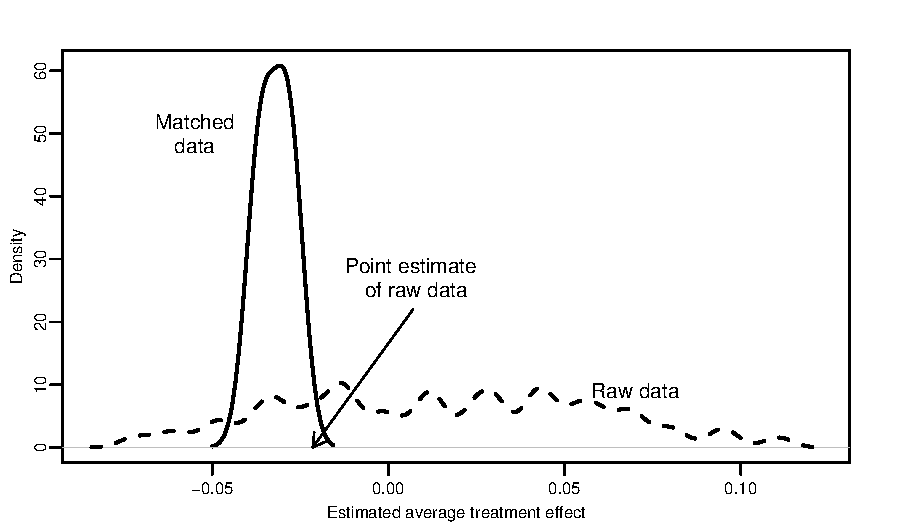
\includegraphics[height=3.5in,angle=0]{figs/kochdens.pdf}
  \end{center}
  \vspace{-0.275in}
  \caption{Density estimates of estimated effects of being
    a highly visible female Republican candidate across 63 possible
    specifications with the Koch data.  The solid line presents
    estimates for the full dataset and the dashed line presents
    estimates for the matched dataset (via subclassification).  The
    vertical arrow presents the point estimate of the regression
    presented in the original paper.  This figure shows that treatment
    effect estimates are much more sensitive to model specification
    for the full dataset compared to the matched dataset.}
  \label{fg:kochdens}
\end{figure}

We now assess the claim of model sensitivity by reporting treatment
effect estimates of parametric models with the full dataset and our
matched (subclassified) dataset.  Specifically, we consider all 63
possible combinations in which the 6 covariates may enter the
regression with the treatment indicator.  For each specification, we
record the point estimate of the treatment coefficient representing
the average effect of being a visible female (Republican) candidate on
the voter's ideological assessment.  For the matched dataset, we run
the exact same specification locally within each subclass, aggregating
the point estimates weighed by the number of treated units in each
subclass.  The result is a distribution of treatment effect estimates
across possible specifications for raw and pre-processed data.

Figure~\ref{fg:kochdens} presents the results, plotting densities of
estimated treatment effects for the raw and pre-processed data.  As
hypothesized, the range of treatment effect estimates is substantially
more variable for the raw data.  Effect estimates, plotted by the
solid line, range from $-0.64$ to $-0.2$, signifying female visibility
causes voters to perceive candidates as more liberal.  The point
estimate from the full data that controls for all six covariates,
signified by the vertical arrow, appears conservative compared to this
range.  Yet estimates from the pre-processed data stand in stark
contrast the to estimates from the raw data.  The range of coefficient
estimates is substantially smaller, ranging from $-0.31$ to $-0.07$,
and the variance across specifications is more than six times smaller
than for the raw data, as shown by the highly peaked density.  Rather
than erring on the conservative side, the reported point estimate now
appears to be substantially larger in substantive effect than we might
expect from the pre-processed data.

In short, not only can pre-processing reduce model dependence,
decreasing the probability that researchers may inadvertently present
unrepresentative estimates, but pre-processing also may change
substantive conclusions of the research.  The fact that treatment
effects may be substantially smaller may even further bolster the
claim that ``[t]he contradictory nature of . . . [the] cues received
from Republican female candidates presents citizens with a complicated
information-processing task'' \citep[p. 460]{Koch02}.

\section{What Can Go Wrong}

\section{Concluding Remarks}

\appendix
\section{Matching Software}\label{s:matchit}

We have created software called MatchIt for the free and open source
package R (see http://www.r-project.org).  MatchIt, which is available
at http://gking.harvard.edu/matchit/, implements a large fraction of
the matching procedures suggested in the diverse scholarly literatures
on this subject.  Most of our software operates with a single command
that takes an existing dataset and produces as output a single
preprocessed matched dataset.  The preprocessed matched dataset can
then be used by other software just as you would have used the
original dataset.

For example, to use propensity score matching of a treatment
indicator, \texttt{treat}, and three pretreatment covariates, we could
use this command:
\begin{verbatim}
match.out <- matchit(treat ~ age + educ + black, data = lalonde)
\end{verbatim}
and to exact match use:
\begin{verbatim}
match.out <- matchit(treat ~ age + educ + black, exact=TRUE, data = lalonde)
\end{verbatim}
Numerous other options are also available.

MatchIt also works well with the general purpose statistics package
Zelig (see http://gking.harvard.edu/zelig).  For example, suppose we
first used MatchIt to subclassify into 5 classes by the propensity
score, use
\begin{verbatim}
match.out <- matchit(treat ~ age + educ + black, subclass=5, data = lalonde)
\end{verbatim}
Then we could use Zelig to estimate a parametric model (in this case
least squares regression) within each of the five subclasses defined
by MatchIt, using data from the control group:
\begin{verbatim}
z.out <- zelig(re78 ~ pscore, model = "ls", by = "psclass", 
                data = match.data(match.out, "control"))
\end{verbatim}
and then set the explanatory variables to predict the potential
outcomes for the treatment group and simulate quantities of interst:
\begin{verbatim}
x.out <- setx(z.out, data = match.data(match.out2, "treat"), cond = TRUE)
s.out <- sim(z.out, x = x.out)
\end{verbatim}


\baselineskip=0.637\baselineskip \bibliographystyle{apsr}
\bibliography{gk,gkpubs}

\end{document}
